\chapter {Detailed problem formulation}\label{ch:problemFormulation3D}
\section{Introduction}\noindent
Given a partially known world, a mission plan, and a small UAV equipped with a LiDAR sensor derive a safe and approach to real-time reactive obstacle avoidance strategy with a small computational footprint compatible with the low computational power available in small UAVs. The main application consists of terrain avoidance for low altitude flights. Following assumption holds:

\noindent
Following issues need to be addressed in practical implementation:
\begin{enumerate}
    \item \textit{Address thick data flow from LiDAR sensor} through Field Of Vision segmentation.
    \item \textit{Derive fast approximation of the reach space $R[\tau,t_0,\vec{x}_0]$ assessment} based on numeric approximation of linearized model.
    \item \textit{Real-time assessment of avoidance situation} based on reachable space $R[\tau,t_0,\vec{x}_0]$ and global goal $\mathscr{WP}_{goal}$.
    \item \textit{Determine escape route in reachable space $R[\tau,t_0,\vec{x}_0]$ search} via expanding search tree.
\end{enumerate}
\noindent
The integration of the proposed reactive obstacle avoidance framework into a UAV flight control framework is described next with reference to Figure \ref{fig:ControlConcept}, similar to $\mathscr{FOV}_{2D}$ and holds its validity:
\begin{itemize}
    \item The \textit{Emergency avoidance module} is invoked to override the trajectory tracking controller when a safety condition is violated.
    \item The \textit{Control strategy switch} will override control input of system and starts avoidance maneuver to achieve \textit{reactive avoidance}.
\end{itemize}
\newpage\noindent
Functional decomposition of the reactive obstacle avoidance framework similar to $\mathscr{FOV}_{2D}$ holds its validity:
\begin{enumerate}
    \item \textit{Obstacle Assessment} - FOV is separated into three subspaces: \textit{free space} – space which is directly visible from the vehicle and does not contain an obstacle, \textit{obstacle space} – space which is directly visible from vehicle and contains an obstacle and \textit{Uncertain space}  space in which direct visibility is hindered by obstacle.
    \item \textit{Reachable space assessment} –- free space can be divided into reachable space, which is reachable with system controls and unreachable space.
    \item \textit{Goal determination} –- within a reachable space local goal for path search is determined, safety margins and turn back maneuver are considered.
    \item \textit{Avoidance path}  calculation via an expanding search tree.
    \item \textit{Avoidance execution} via movement automaton.
\end{enumerate}

\section{Simple plane model}\label{sec:3DsimplisticplaneModel}
\noindent For avoidance theorem formulation in three dimensional space simplified rigid body kinematic model will be used. This model have decoupled roll, yaw and pitch angles which enables to provide simpler and more clean control (e.g movements can be simplified). 

\begin{equation}\label{eq:simple3dStatevector}
    \vec{x} = \left [ x_v,y_v,z_v,\alpha_v,\beta_v,\gamma_v \right ]^T
\end{equation}
State vector (\ref{eq:simple3dStatevector}) defined as positional state in euclidean position in right-hand euclidean space, where $x_v, y_v,z_v$ states, for latitude, longitude and altitude. Orientation angles for vehicle are $\alpha\beta,\gamma$ for roll, pitch, yaw angle.
\begin{equation}\label{eq:simple3dInputVector}
    \vec{u} = \left [ v, \omega_{\alpha_v}, \omega_{\beta_v},\omega_{\gamma_v}\right ]^T
\end{equation}
Input vector (\ref{eq:simple3dInputVector}) is defined as frontal velocity of vehicle $v$,orientation change in main axes as angular speed $\omega_{\alpha_v},\omega_{\beta_v},\omega_{\gamma_v}$
\begin{equation}\label{eq:simple3dvelocityDistribution}
    \begin{bmatrix}
    v_x\\
    v_y\\
    v_z\
    \end{bmatrix}
    = R_{XYZ}(\alpha_v,\beta_v,\gamma_v)
    \begin{bmatrix}
    v\\
    0\\
    0
    \end{bmatrix}
    =
    \begin{bmatrix}
        f_{v_x}(v,\alpha_v,\beta_v,\gamma_v)\\
        f_{v_y}(v,\alpha_v,\beta_v,\gamma_v)\\
        f_{v_z}(v,\alpha_v,\beta_v,\gamma_v)\\
    \end{bmatrix}
    =
    \begin{bmatrix}
         v\cos(\beta_v)\cos(\gamma_v)\\
         v\cos(\beta_v)\sin(\gamma_v)\\
         -v\sin(\beta_v)\\
    \end{bmatrix}
\end{equation}
Velocity distribution function (\ref{eq:simple3dvelocityDistribution}) is is defined trough standard rotation matrix (\ref{eq:xyzspaceRotationMatrix}) and frontal velocity $v$, final distributed velocity is time depending function with values $v_x$, $v_y$, $v_z$ given by functions $f_{v_x}(\dots)$, $f_{v_y}(\dots)$,$f_{v_z}(\dots)$. Final nonlinear model which have been derived from reference model \cite{stevens2015aircraft} is defined by (\ref{eq:simple3ddifferentialequations}).\\
\begin{equation}\label{eq:simple3ddifferentialequations}
    \begin{aligned}
        \dot{x}_v &= v_x  =f_{v_x}(v,\alpha_v,\beta_v,\gamma_v) = v\cos(\beta_v)\cos(\gamma_v)\\
        \dot{y}_v &= v_y  =f_{v_y}(v,\alpha_v,\beta_v,\gamma_v) = v\cos(\beta_v)\sin(\gamma_v)\\
        \dot{z}_v &= v_z  =f_{v_z}(v,\alpha_v,\beta_v,\gamma_v) = -v\sin(\beta_v)\\
        \dot{\alpha}_v &= \omega_{\alpha_v}\\
        \dot{\beta}_v &= \omega_{\beta_v}\\
        \dot{\gamma}_v &= \omega_{\gamma_v}\\
    \end{aligned}
\end{equation}   

\newpage
\section{Optimal trajectory planning}
\noindent Avoidance execution takes place in avoidance grid area $\mathscr{A}(t_d)$, where $t_d$ is decision time. Because Movement automaton $\mathscr{MA}$ is used to control plant, this problem can be addressed by discrete search function. Problem can be vaguely formulated as path finding in constrain-ted field of vision. Obstacles and system maneuverability is main constraint. For this part duality, between optimal path and reach sets will be relaxed. Reach set for this section guarantees only existence of trajectory. Reach set method used in section \ref{s:maxReachSet}. guarantees existence of minimal solution, because of reach set and trajectory duality.


\subsection{Optimal control problem formulation}
\noindent\textit{Performance functional} is given as standard cost function formulation for energy consumption line integral of trajectory $[x(t),y(t),z(t)]$ and line integral of steering input $[\beta_v(t),\gamma_v(t)]$  and for penalisation coefficients of steering $[c_\beta,c_\gamma]$ is in continuous time t given as: 
\begin{equation}\label{eq:j01}
    J_S(\vec{x},\vec{u})= \int_{t_0}^{\tau} \sqrt{\dot{x}_v(t)^2 + \dot{y}_v(t)^2 + \dot{z}_v(t)^2} + \sqrt{c_\beta\dot{\beta}_v(t)^2+c_\gamma\dot(\gamma)_v(t)^2} \quad \text{d}t
\end{equation}
For movement automaton sequence $B=\{m_1(t_1),\dots,m_k(t_k)\}$ the trajectory equivalence definition holds similarity property, therefore partially continuous signal generated by execution of movement buffer $B$ at movement automaton $\mathscr{MA}$ is equal to continuous signal given by $u(t)$. Moreover state in case continuous control $x(t)$ is equal to state generated by movement automaton $\mathscr{MA}$. One can rewrite (\ref{eq:j01}) for sequence of movements as $B=\{m_1(t_1),\dots,m_k(t_k)\}$ like follows:
\begin{equation}\label{eq:j02}
    J_S(\vec{x},\vec{u})= \sum_{k=1}^n \int_{t_{k-1}}^{t_{k}} \sqrt{\dot{x}_v(t)^2 + \dot{y}_v(t)^2 \quad \text{d}t + \dot{z}_v(t)^2} + \sqrt{c_\beta\dot{\beta}_v(t)^2+c_\gamma\dot(\gamma)_v(t)^2} \quad \text{d}t
\end{equation}
Execution of movements creates discrete time trail $\{\tau_0,\tau_1,\dots,\tau_k\}$, which marginalizes every time of movement execution start and end. Therefore movement $m_k(t_k)$ have execution period given as $(\tau_{k-1},\tau_k]$. Where $\tau_i$ is discete movement execution time. With some loss of precision one can rewrite (\ref{eq:j02}) as:
\begin{equation}\label{eq:j03}
    J_D(\vec{x},\vec{u}) = \sum_{k=1}^n \sqrt{\begin{aligned}
        &\left(x_v(\tau_{k})-x_V(\tau_{k-1)})\right)^2\\
        +&\left(y_v(\tau_{k})-y_V(\tau_{k-1)})\right)^2\\
        +&\left(z_v(\tau_{k})-z_V(\tau_{k-1)})\right)^2
    \end{aligned}}
    + \sum_{k=1}^n \sqrt{
    \begin{aligned}
        &c_\beta\left(\beta_v(\tau_{k})-\beta_v(\tau_{k-1})\right)^2\\
        +&c_\gamma\left(\gamma_v(\tau_{k})-\gamma_v(\tau_{k-1})\right)^2
    \end{aligned}}
\end{equation}
In given form equation $eq:j03$ uses only norm of distance and steering vectors differentials in execution time $t\in(\tau_{k-1},\tau_{k}]$. For unit movements $m_k\in M$ cost functional for trajectory $f(\dots)$ and cost functional for steering $g(\dots)$ can be proposed:
\begin{equation}\label{eq:j04}
    J_D(\vec{x},\vec{u}) = \sum_{k=1}^n f(m_k,\vec{x}_k,\vec{x}_{k-1}) + g(m_k,\vec{x}_k,\vec{x}_{k-1},c_\beta,c_\gamma)
\end{equation}
Functional $f(\dots)$ yields similar values for movement $m_k$ independent of his order in movement sequence $B$, therefore it can be approximated by mapping function $\hat{f}(mi)$:
\begin{equation}\label{eq:apff}
    f(m_k,\vec{x}_k,\vec{x}_{k-1})= \sqrt{\begin{aligned}
        &\left(x_v(\tau_{k})-x_V(\tau_{k-1)})\right)^2\\
        +&\left(y_v(\tau_{k})-y_V(\tau_{k-1)})\right)^2\\
        +&\left(z_v(\tau_{k})-z_V(\tau_{k-1)})\right)^2
    \end{aligned}}
    \sim \hat{f}(m_k)
\end{equation}
Functional $g(\dots)$ yields similar values for movement $m_k$ independent of his order in movement sequence $B$, therefore it can be approximated by mapping function $\hat{g}(m_k)$:
\begin{equation}\label{eq:apfg}
    g(m_k,\vec{x}_k,\vec{x}_{k-1},c_\beta,c_\gamma) = \sum_{i=1}^k \sqrt{
    \begin{aligned}
        &c_\beta\left(\beta_v(\tau_{k})-\beta_v(\tau_{k-1})\right)^2\\
        +&c_\gamma\left(\gamma_v(\tau_{k})-\gamma_v(\tau_{k-1})\right)^2
    \end{aligned}}
    \sim \hat{g}(m_k)
\end{equation}
Cost function (\ref{eq:j03}) is equivalent to cost function (\ref{eq:j04}). Transition period in simple systems like (\ref{eq:simple3ddifferentialequations}). \textit{Dynamic movement primitives} $p_i$ have minimal impact on system state $\vec{x}(t)$ and system input $\vec{u}(t)$ have minimal impact on movement cost $m_k(t_k)$ cost. With approximation functional $\hat{f}(\dots)$ (\ref{eq:apff}) and $\hat{g}(\dots)$ (\ref{eq:apfg}), cost function (\ref{eq:j04}) can be written as:
\begin{equation}\label{eq:j05}
    \hat{J}_D(\vec{x},\vec{u}) = \sum_{k=1}^n \hat{f}(m_k) + \hat{g}(m_k)
\end{equation}
For system given by (\ref{eq:simple3ddifferentialequations}) it is possible to show that continuous cost $J_S$ (\ref{eq:j01}), discrete cost $J_D$ (\ref{eq:j03}) and approximated discrete cost $\hat{J}_D$ (\ref{eq:j05})are equal:
\begin{equation}
    J_S(\vec{x},\vec{u}) \sim J_D(\vec{x},\vec{u})\sim \hat{J}_D(\vec{x},\vec{u}) = \sum_{k=1}^n \hat{f}(m_k) + \hat{g}(m_k)
\end{equation}

\noindent\textit{Constraints} are given by reachable space in avoidance grid $\mathscr{A}(t_0)$. Let $\mathscr{R}(t_0,\vec{x}_0)\subseteq \mathscr{A}(t_0)$ be reachable space at beginning of avoidance. Cell $c_g\in\mathscr{R}(t_0,\vec{x}_{0})$ is reachable cell and it has been determined as goal of avoidance. At initial state $\vec{x}(t_0)$ at decision time $t_d$. For trajectory $\mathscr{T}(B,c_0)$ there is sufficient control constraint given by $\mathscr{T}(B,t_0)\in \mathscr{R}(t_0)$. Therefore movement chain $B\in M^k$ given as series of movements $\{m_1(t_1),\dots,m_k(t_k)\}$ is constrained by following constraint:
\begin{equation}
    \left\{\mathscr{A}(t_0)-\mathscr{R}(t_0,\vec{x}_0)\right\} \cup \mathscr{T}(B,\vec{x}_0) = \{\},\quad B\in M^k
\end{equation}
\noindent Because cell $c_g$ is member subspace of reachable set $\mathscr{R}(t_0,\vec{x}_0)$. Trajectory existence from initial state $\vec{x}(t_0)$ to space occupied by goal cell $c_g$ is guaranteed.
\textit{Stop condition} for trajectory search is reaching center of cell $[x_c,y_c,z_c]$ with system position:
\begin{equation}
    \norm{[\vec{x}_g - \vec{x}(\tau_k)]} \le d_{stop},\quad \vec{x}(\tau_k)\in\mathscr{T}(x_0).
\end{equation}
Where $\vec{x}_g$, is center of cell $c_g$, $\vec{x}(\tau_k)$ is system position on trajectory $\mathscr{T}(B,\vec{x}_0)$ after execution of buffer $B={m_1,\dots,m_k}$ at time $\tau_k$.

\textit{Initial state} is equal to system initial state at time of decision $\vec{x}_0=\vec{x}(t_0)=\vec{x}(t_d)$. Initial input state is equal to input state at time of decision $\vec{u}_0=\vec{u}(t_0)=\vec{u}(t_d)$.

\textit{Control constraint} for system maximal steering angles are given: 
\begin{equation}
    \beta_v(t)\in [\beta_{min},\beta_{min}]    
\end{equation}
\begin{equation}
    \gamma_v(t)\in [\gamma_{min},\gamma_{min}]    
\end{equation}
\newpage\noindent \textit{Problem formulation} is stated like follow:
\begin{itemize}
    \item For system given by $\dot{x} = f(\vec{x},\vec{u})$ with initial state $x_0$ and control $\vec{u}_0$.
    \item Find optimal trajectory $\mathscr{T}(B,\vec{x}_0)$ which stays in reach set $\mathscr{R}(t_0,\vec{x}_0)$ and reaches goal cell $c_g$.
    \item Minimize cost functional $\hat{J}_D(\vec{x},\vec{u})$.
    \item With given control constraints and movement automaton $\mathscr{MA}$ as control.
\end{itemize}
Trajectory search problem can be simplified to movement buffer search $B\in M^k$ which holds constraints of state and input. 

\subsection{Minimum principle}
\noindent Reach set $\mathscr{R}(t_0,\vec{x}_0)$ guarantees that at least one solution exists. Reach set $\mathscr{R}(t_0,\vec{x}_0)$ is closed compact set within state space $\vec{x}\in\R^n$, therefore amount of trajectories $\mathscr{T}(B,\vec{x}_0)$ is finite. Not every trajectory $\mathscr{T}(B,\vec{x}_0)$ ends in goal cell $c_g\in\mathscr{A}(t_i)$. Each trajectory $\mathscr{T}$ is defined by buffer $B$, which contains chain of movements $\{m_1(t_1),\dots,m_k(t_k)\}$. Let say that $i$ is maximal count of movements to escape reach set $\mathscr{R}(t_0,\vec{x}_0)$. Then length of movement chain $B$ have following property:
\begin{equation}
    B=\{m_1(t_1),\dots,m_k(t_k)\},\quad|B|\le i
\end{equation}
With preposition that permutation set of movement buffers, in given constraint have finite count of members, e. g. is countable, standard permutation technique can be used to obtain  minimal trajectory. Depending on avoidance grid size $\mathscr{A}(t_i)$ this can take factorial amount of computation time.

Original cost function $\hat{J}_D$ (\ref{eq:j05}) does not contain terminal cost. If expected terminal cost is introduced standard A* search function can be used. Depending on implementation A* search can achieve logarithmic complexity and its more feasible for on-line optimisation. Let say that trajectory $\mathscr{T}(B,x_0)$ brings system to state $x(\tau_k)$, position of this state is given by $\vec{p}_v=[x_\tau,y_\tau,z_\tau]$ and center of goal cell $c_g$ is given as $\vec{p}_g=[x_g,y_g,z_g]$. then terminal cost of system at time $\tau_k$ is given:
\begin{equation}\label{eq:j06}
    J_T(\vec{x},\vec{u},c_g) = \norm{\vec{p}_v-\vec{p}_g}
\end{equation}
Final cost function is given as combination travel cost function $\hat{J}_D(\vec{x},\vec{u})$(\ref{eq:j05}) and terminal cost function $J_T(x,u,c_g)$ (\ref{eq:j05}). One can write final cost functional as:
\begin{equation} \label{eq:j07}
    J(\vec{x},\vec{u},c_g) = \norm{\vec{p}_v-\vec{p}_g} + \sum_{k=1}^n \hat{f}(m_k) + \hat{g}(m_k)
\end{equation}
Minimum principle implementation for (\ref{eq:j07}) cheapest path search is given by following section.

\subsection{Rapid exploraiton path search}
\noindent Rapid path exploration method is method for finding feasible paths in known environment based on limited system dynamics $\dot{x}=f(\vec{x},\vec{u})$ where input belongs to control  set $\vec{u}(t)\in U(T)$, example can be seen in figure \ref{fig:58rapidPathExploaation}.
\begin{figure}[H]
    \centering
    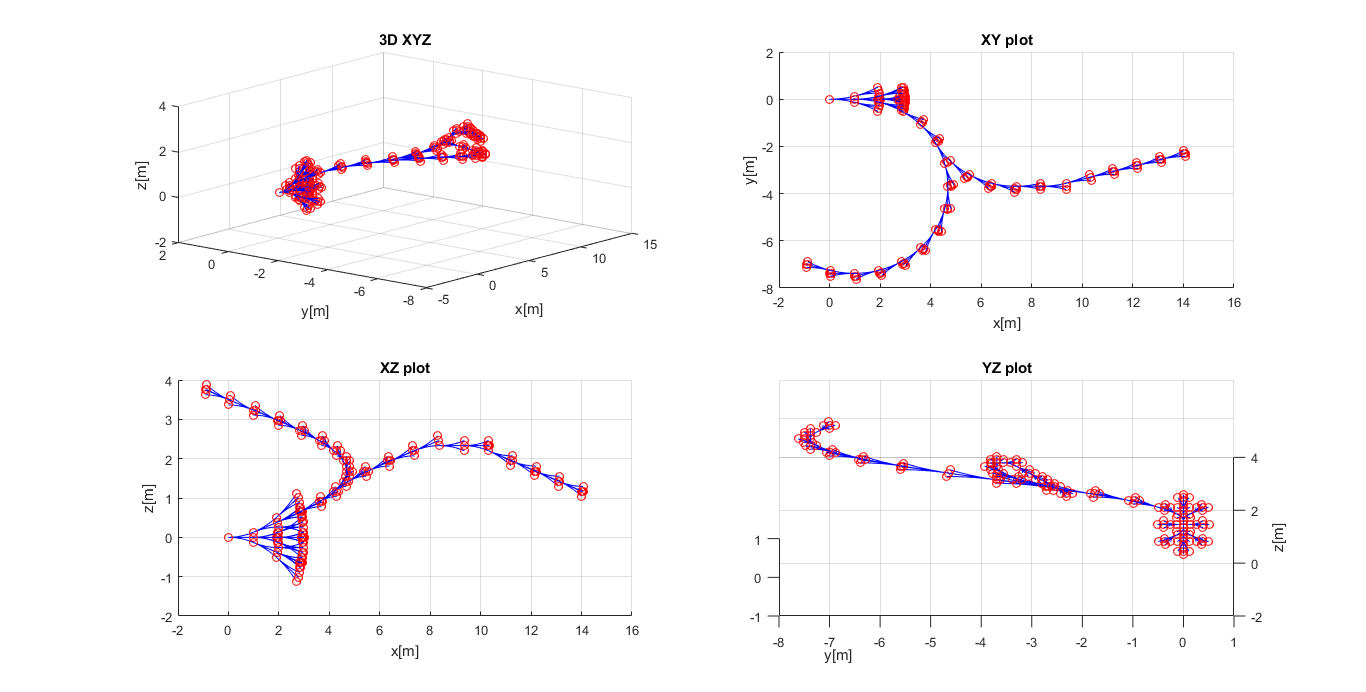
\includegraphics[width=\linewidth]{\FIGDIR/58_Rapid_exploration_path_tree.png}
    \caption{Rapid path exploration tree example with cost function $\hat{J}_D$(\ref{eq:j07}).}
    \label{fig:58rapidPathExploaation}
\end{figure}
\noindent Algorithm is based on tree search of possible movement nodes which represents vehicle state snapshots $x(t_i) i\in \N^+$. State snapshots are calculated based on predictive or linear model, to save computation time and calculation guarantees that real vehicle state $\hat{x}(t_i)$ will reach  state $\vec{x}(t_i)$ with small perturbation $\epsilon$ therefore for each predicted state following inequality holds:
\begin{equation}\label{eq:marginalErrorofPrediction}
    \norm{\hat{x{t_i}}-\vec{x}(t_i)}\le \epsilon^i,\quad i \in \N^+
\end{equation}
\noindent All possible trajectories $\mathscr{T}$ in search tree are represented as sequence of nodes. Each node have defined parent, which is reference to previous node and leafs which are references to possible followers in path. For our purpose augmented data structure \textit{Node} will be presented with following properties:
\begin{enumerate}
    \item \textit{Movement} - movement which has been executed on this node.
    \item \textit{Goal distance} - distance to goal point in space calculated by (\ref{eq:distanceToGoalCalc}).
    \item \textit{Explored} - indication if node have been explored by stack execution true or false.
    \item \textit{Vehicle} - vehicle structure with state and obstacles situation.
    \item \textit{Parent} - parent node handle, if empty node is root of tree. 
    \item \textit{Leafs} - list of accessible non vehicle destructive leafs.
\end{enumerate}
\begin{equation}\label{eq:distanceToGoalCalc}
    d_{goal}(vehicle,\mathscr{W}_g) = 
    \begin{cases}
        \norm{\vec{x}_v-\vec{x}_{goal}}&:\nexists o \in \mathscr{O}; o.danger = 1 \vee 2\\
        \infty&:otherwise
    \end{cases}
\end{equation}
\noindent For purpose of rapid exploration limited move set needs to be introduced, therefore based on defined simplistic system model control set (\ref{simple3dControlSet}):
\begin{equation}\label{eq:rapidExplorationMovementSet}
    moveSet=
    \begin{cases}
        \left\{straight,left,right,up,down \right\} &: node.movement == straight\\
        \left\{straight,left, \right\} &: node.movement == left\\
        \left\{straight,right \right\} &: node.movement == right\\
        \left\{straight,up \right\} &: node.movement == up\\
        \left\{straight,down \right\} &: node.movement == down
    \end{cases}
\end{equation}
\noindent Goal of rapid exploration is to cover maximum amount of space without redundancy therefore allowed movement set \ref{eq:rapidExplorationMovementSet} is covering this situation. For example movement series $[right,left]$ returns to path given by movement series $[straight,straight]$, therefore possible movements after i finis $right$ movement are $right,straight$. This rule reduces search tree complexity from branching factor $n^5$ to branching factor $n^3$. Expand function represented by algorithm \ref{alg:03}.

\begin{algorithm}[H]
\caption{Node expand(...) function.}
\label{alg:03}
\SetKwInOut{Input}{Input}\SetKwInOut{Output}{Output}
\Input{Node node}
\Output{Node[] leafs}
\If{isEmpty(node.leafs)}{
    \ForEach{$appliedMovement\in \left\{straight,left,right,up,down \right\}$}{
        newVehicle = vehicle.predictPosition(appliedMovement);\\
        Node child = new Node(vehicle);\\
        child.recalculateDistance();\\
        child.parrent = node;\\
        node.leafs.append(child);
    }
}
\end{algorithm}
\noindent Node selection is executed based on algorithm \ref{alg:04}. Not all leafs of expanded node can be exploration candidates, because some movements can lead to vehicle crash, which is represented by $node.goalDistance = \infty$. Other reason to decline leaf as exploration candidate is inappropriate movement, movement set which is based on parent node movement (\ref{eq:rapidExplorationMovementSet}), can allow only certain candidates to be explored. Other selection criteria based on system dynamics or constraints can be introduced into selection function later.

\begin{algorithm}[H]
    \caption{Node select(...) function.}
    \label{alg:04}
    \SetKwInOut{Input}{Input}\SetKwInOut{Output}{Output}
    \Input{Node node}
    \Output{Node[] candidates}
    candidates = [];\\
    \ForEach{leaf $\in$ node.leafs}{
    \If{leaf.movement $\in$ moveSet and leaf.goalDistance $\neq \infty$ and\\
        leaf.goalDistance $\le$ node.goalDistance and leaf.explored == false}{
            leaf.explored = true;\\
            candidates.append(leaf);
    }
}
\end{algorithm}
\noindent Stack structure search is used for heuristic search of optimal path according to cost function (\ref{eq:j07}). Path given by heuristic algorithm \ref{alg:05}. is semi-optimal strongly depending on chosen time interval $t_i$ for prediction, count of predicted states $i$ and acceptable marginal error of prediction (\ref{eq:marginalErrorofPrediction}). 
\begin{algorithm}
    \caption{Search path function.}
    \label{alg:05}
    \SetKwInOut{Input}{Input}\SetKwInOut{Output}{Output}
    \Input{Node root, $\mathscr{WP}$ goal}
    \Output{Node path}
    stack = [root];
    \While{~isEmpty(stack)}{
        node = findBestCandidate(stack,goal); (\ref{eq:j07})\\
        node.expand($\dots$); (alg. \ref{alg:03}.)\\
        candidates = node.select($\dots$); (alg. \ref{alg:04}.)\\
        \ForEach{candidate $\in$ candidates}{
            \If{candidate.distance(goal) $\le$ marginDistance}{
                return candidate;
            }
        }
    }
\end{algorithm}
